\subsection{Direct search methods}\label{direct-search}
Among direct search methods, we will describe the \textit{generalized pattern search} (hereafter GPS) method \cite{Audet2002} and the \textit{mesh adaptive direct search} (hereafter MADS) method \cite{Audet2006}.

To describe the GPS algorithm, it is necessary to define a mesh, which is used to describe the search sets within the GPS algorithm. Let $ \mathbf{G} \in \mathbb{R}^{n \times n} $ be invertible and $ \mathbf{Z} \in \mathbb{Z}^{n \times p} $, $n, p \in \mathbb{N}$. Assume that every vector from $ \mathbb{R}^{n} $ can be expressed as a linear combination of the columns of matrix $ \mathbf{Z} $ (treated as vectors), such that all the coefficients in this linear combination are non-negative. Furthermore, let $ \mathbf{D} = \mathbf{G} \mathbf{Z} $. The mesh $ \mathbf{M} $ generated by $ \mathbf{D} $ centered at point $ \vec{x} $ is defined as
\begin{equation}
	\mathbf{M} = \left\{ \vec{x} + \delta \, \mathbf{D} y \, | \, y \in \mathbb{N}^p \right\},
\end{equation}
where $ \delta $ is called the mesh size parameter \cite{BBO-textbook, Audet2002}. In each iteration of the GPS algorithm, the shape of the mesh generally changes, as it is always centered at the point representing the best estimate in that iteration, and the size of the mesh step also changes. Let $ \vec{x}_k $ and $ \delta_k $ represent the estimate of the solution and the mesh size in the $ k $-th iteration, respectively. We 
then define the mesh in the $ k $-th iteration, denoted as $ \mathbf{M} _k $, as
\begin{equation}
	\mathbf{M} _k = \left\{ \vec{x}_k + \delta_k \, \mathbf{D} y \, | \, y \in \mathbb{N}^p \right\}.
\end{equation}
Note that the columns of matrix $ \mathbf{D} $, as defined above, can be interpreted as the possible directions in which the GPS algorithm searches the optimization space \cite{BBO-textbook, Audet2002}. Examples of search directions and meshes generated by different matrices $\mathbf{G}$ and $\mathbf{Z}$ are presented in Figure~\ref{fig:gps}.


\begin{figure}[H]
	\centering
	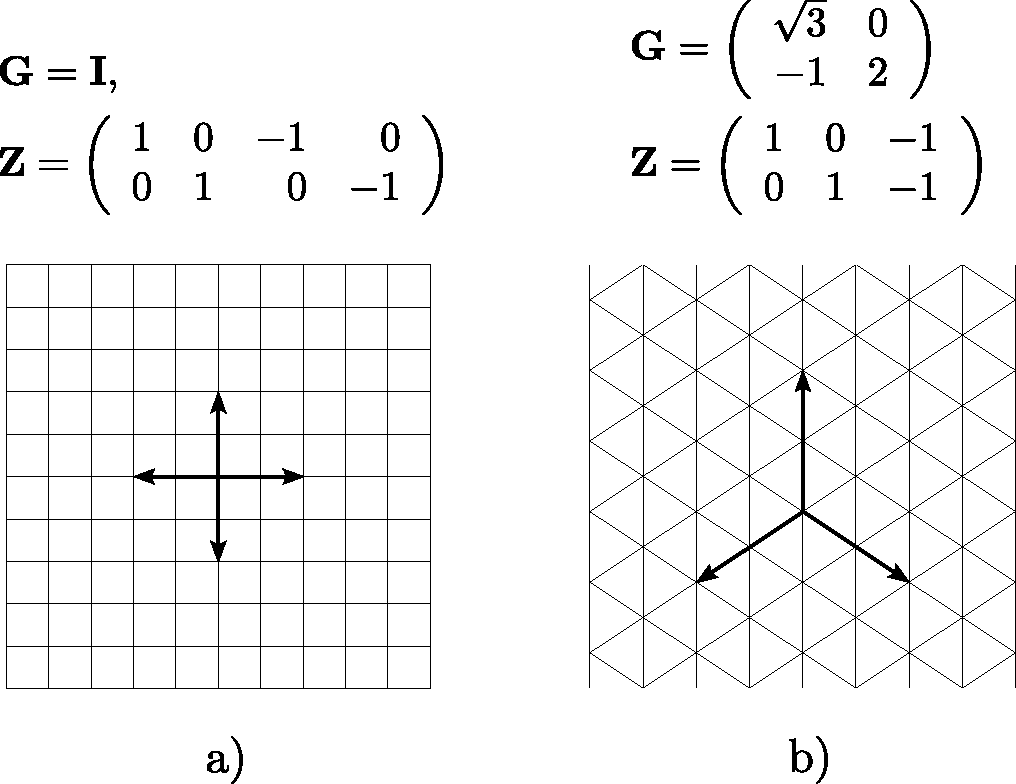
\includegraphics[width=0.70\textwidth]{figures/gps.pdf}
	\caption{Examples of search directions and meshes in $\mathbb{R}^2$ with
		obtained by different choices of $\mathbf{G}$ and~$\mathbf{Z}$. The mesh points
		are at the intersections of the lines, the arrows represent possible search directions.}
	\label{fig:gps}
\end{figure}


After initializing the necessary starting parameters, each iteration of the GPS algorithm is divided into two main steps. The first step is called the search step. During the search step, a finite set $S_k$ of candidate mesh points, selected according to a strategy specified by the user, is evaluated by computing the objective function at each one of the points. If none of the evaluated points represents an improvement over the value $ f(\vec{x}_k) $, the poll step follows. In the poll step, the objective function is evaluated at all neighboring mesh points of $ \vec{x}_k $. The poll set in $k$-th iteration is defined as $P_k = \{x_k + \delta_k d \, | \, d \in \mathbf{D}\}$. If none of the evaluated points represents an improvement over the value $ f(\vec{x}_k) $, we set $ \vec{x}_{k+1} = \vec{x}_k $ and decrease the mesh size, i.e., $ \delta_{k+1} < \delta_k $. However, if a point that improves the estimate of the solution is found in either the search or the poll step, this point is set as $ \vec{x}_{k+1} $, and the mesh size is increased, i.e., $ \delta_{k+1} > \delta_k $~\cite{BBO-textbook, Audet2002}.

The changes described above define a new mesh $ \mathbf{M} _k $ in each iteration. The mesh changes throughout the GPS algorithm. The algorithm terminates when $ \delta_{k+1} < \varepsilon $ for some user-specified $ \varepsilon > 0 $. It can be shown that the mesh step converges to zero, and under appropriate assumptions, the solution estimates converge to a stationary point of the objective function. Details can be found in \cite{BBO-textbook}. It should be noted that the convergence of GPS has been proven for unconstrained problems \cite{BBO-textbook}. The full GPS algorithm is presented in Algorithm~\ref{GPS-algo}.
\\[4pt]
\begin{algorithm}[H]
	\caption{Generalized Pattern Search (GPS) for unconstrained optimization}\label{GPS-algo}
	\begin{algorithmic}[1]
		\Require Function $f: \mathbb{R}^n \to \mathbb{R}$, initial point $x_0$, initial mesh size parameter $\delta_0$, positive spanning matrix $\mathbf{D}$, mesh size adjustment parameter $\tau \in (0, 1)$, stopping tolerance $\epsilon_{\text{stop}}$, iteration counter $k \gets 0$
		\Ensure Approximate solution $x^*$
		
		\Procedure{GPS}{$x_0$}
		
		\While{$\delta_k > \epsilon_{\text{stop}}$}
		
		\Algphase{1. Search}
		\State Define a finite subset $S_k$ of the mesh $\mathbf{M}_k$
		\If{$f(t) < f(x_k)$ for some $t \in S_k$}
		\State Set $x_{k+1} \gets t$ and $\delta_{k+1} \gets \tau^{-1} \delta_k$
		\State \textbf{continue}
		\Else
		\State Go to Poll step
		\EndIf
		
		\Algphase{2. Poll}
		\State Select a positive spanning set $\mathbf{D}_k \subseteq \mathbf{D}$
		\State Define $P_k = \{x_k + \delta_k d : d \in \mathbf{D}_k\}$
		\If{$f(t) < f(x_k)$ for some $t \in P_k$}
		\State Set $x_{k+1} \gets t$ and $\delta_{k+1} \gets \tau^{-1} \delta_k$
		\Else
		\State $x_k$ is a mesh local optimizer
		\State Set $x_{k+1} \gets x_k$ and $\delta_{k+1} \gets \tau \delta_k$
		\EndIf
		
		\Algphase{3. Termination}
		\If{$\delta_{k+1} \leq \epsilon_{\text{stop}}$}
		\State \textbf{terminate}
		\Else
		\State Increment $k \gets k+1$ and continue
		\EndIf
		
		\EndWhile
		\EndProcedure
	\end{algorithmic}
\end{algorithm}

We now turn our attention to the MADS algorithm, which generalizes the GPS algorithm by allowing for a different set of polling directions. The key difference is that MADS introduces the concept of a frame, which allows the poll directions to form a dense subset in $ \mathbb{R}^{n} $ as the algorithm progresses~\cite{BBO-textbook, derivative-free-review}. The frame $\mathbf{F}_k$ at iteration $k$ is defined as
\begin{equation}
	\mathbf{F}_k = \{ \vec{x} \in \mathbf{M}_k \ \big| \ \| \vec{x} - \vec{x}_k \|_\infty \leq \Delta_k b \},
\end{equation}
where $M_k$ represents the current mesh, $ \Delta_k $ is the frame size parameter, satisfying $ \delta_k \leq \Delta_k $, and $b = \max \ \{ \| d \| _\infty \ \big| \ d \in \mathbf{D} \}$. The extent of the frame is determined by the parameter $ \Delta_k $, and the polling directions are taken from this frame.

Each iteration of the MADS algorithm begins similarly to GPS, with a search step where a finite set $S_k$ of candidate points, selected based on the current mesh, is evaluated by computing the objective function at each of the points. If none of these points improves upon the current best solution, the algorithm proceeds to the poll step. 
 
The poll set $P_k$ is a subset of points selected from $\mathbf{F}_k$ and $\mathbf{M}_k$. Trivially, $P_k \subseteq \mathbf{F}_k \subseteq \mathbf{M}_k$. Importantly, the mesh size parameter $ \delta_k $ is allowed to decrease more rapidly than the  enabling the poll directions to asymptotically become arbitrarily dense~\cite{Audet2006}. This aspect is crucial, as it ensures that MADS can explore directions in a finer and more systematic manner than GPS, leading to better convergence properties.


\begin{figure}[H]
	\centering
	\vspace{0.5cm}
	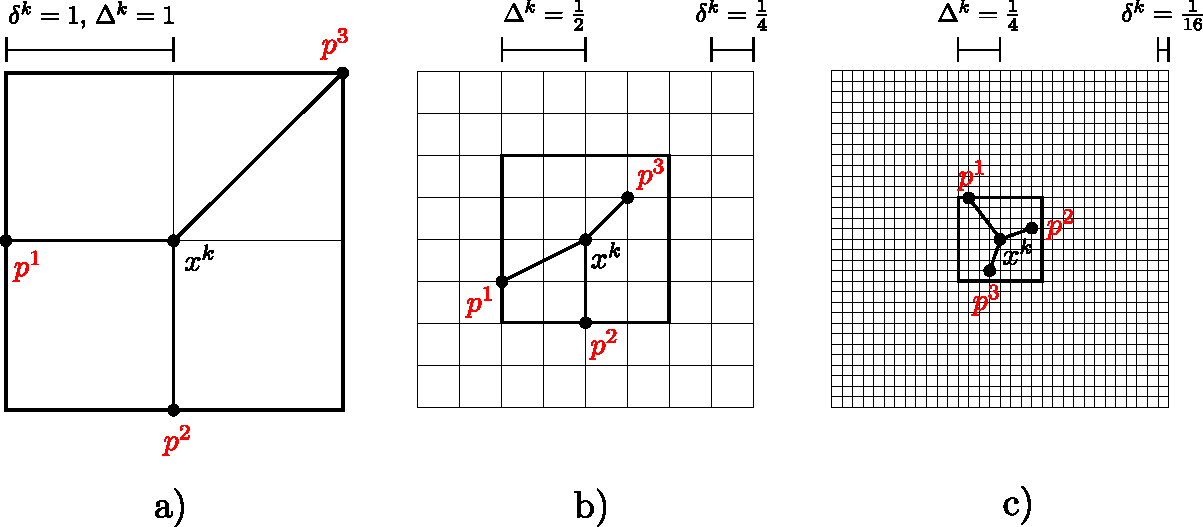
\includegraphics[width=1.01\textwidth]{figures/mads.pdf}
	\caption{Examples of meshes and frames $\mathbb{R}^2$ for different
		values of $\delta_k$ and $\Delta_k$}
	\label{fig:mads}
\end{figure}

If an improvement is found in the poll step, the new point is set as $ \vec{x}_{k+1} $, and the frame size $ \Delta_k $ and mesh size $ \delta_k $ may be increased to encourage further exploration. Conversely, if no improvement is found, $ \vec{x}_{k+1} = \vec{x}_k $, and the mesh size is reduced, i.e., $ \delta_{k+1} < \delta_k $, to allow for a more local search. The process of shrinking and refining the frame and mesh sizes continues until $ \delta_k $ falls below a user-specified threshold, at which point the algorithm terminates.

MADS also incorporates the \textit{extreme barrier function} to handle constraints, similarly to GPS. For constrained optimization problems, the objective function is modified into an extreme barrier function~\cite{BBO-textbook}, which penalizes any infeasible points by assigning them an infinite objective value. This simple yet effective strategy ensures that the optimization remains focused on feasible regions of the search space, and the algorithm converges to a stationary point even for constrained problems. A full description of the MADS algorithm and its implementation details can be found in~\cite{BBO-textbook}.



\begin{algorithm}[H]
	\caption{Mesh Adaptive Direct Search (MADS)}\label{MADS}
	\begin{algorithmic}[1]
		\Require Function $f_{\infty}: \mathbb{R}^n \to \mathbb{R} \cup \{\infty\}$, initial point, initial frame size parameter $\Delta_0$, positive spanning matrix $\mathbf{D}$, mesh size adjustment parameter $\tau \in (0,1)$, stopping tolerance $\epsilon_{\text{stop}}$, iteration counter $k \gets 0$
		\Ensure Approximate solution $x^*$
		
		\Procedure{MADS}{$x_0$}
		
		\While{$\Delta_k > \epsilon_{\text{stop}}$}
		
		\Algphase{1. Parameter Update}
		\State Set the mesh size parameter $\delta_k = \min \{\Delta_k, (\Delta_k)^2\}$
		
		\Algphase{2. Search}
		\State Define a finite set $S_k \subset \mathbf{M}_k$ such that:
		\If{$f_{\infty}(t) < f_{\infty}(x_k)$ for some $t \in S_k$}
		\State Set $x_{k+1} \gets t$ and $\Delta_{k+1} \gets \tau^{-1}\Delta_k$
		\State \textbf{continue}
		\Else
		\State Go to Poll step
		\EndIf
		
		\Algphase{3. Poll}
		\State Select a positive spanning set $\mathbf{D}_{k}$ and define:
		\State $P_k = \{x_k + \delta_k d : d \in \mathbf{D}_{k}\}$, a subset of the frame $\mathbf{F}_k$ with extent $\Delta_k$
		\If{$f_{\infty}(t) < f_{\infty}(x_k)$ for some $t \in P_k$}
		\State Set $x_{k+1} \gets t$ and $\Delta_{k+1} \gets \tau^{-1}\Delta_k$
		\Else
		\State Set $x_{k+1} \gets x_k$ and $\Delta_{k+1} \gets \tau\Delta_k$
		\EndIf
		
		\Algphase{4. Termination}
		\If{$\Delta_{k+1} \leq \epsilon_{\text{stop}}$}
		\State \textbf{terminate}
		\Else
		\State Increment $k \gets k+1$ and continue
		\EndIf
		
		\EndWhile
		\EndProcedure
	\end{algorithmic}
\end{algorithm}